%
% main.tex -- Paper zum Thema <helmholtz>
%
% (c) 2020 Autor, OST Ostschweizer Fachhochschule
%
% !TEX root = ../../buch.tex
% !TEX encoding = UTF-8
%
\chapter{Thema\label{chapter:helmholtz}}
\kopflinks{Thema}
\begin{refsection}
\chapterauthor{Hans Muster}

Ein paar Hinweise für die korrekte Formatierung des Textes
\begin{itemize}
\item
Absätze werden gebildet, indem man eine Leerzeile einfügt.
Die Verwendung von \verb+\\+ ist nur in Tabellen und Arrays gestattet.
\item
Die explizite Platzierung von Bildern ist nicht erlaubt, entsprechende
Optionen werden gelöscht. 
Verwenden Sie Labels und Verweise, um auf Bilder hinzuweisen.
\item
Beginnen Sie jeden Satz auf einer neuen Zeile. 
Damit ermöglichen Sie dem Versionsverwaltungssysteme, Änderungen
in verschiedenen Sätzen von verschiedenen Autoren ohne Konflikt 
anzuwenden.
\item 
Bilden Sie auch für Formeln kurze Zeilen, einerseits der besseren
Übersicht wegen, aber auch um GIT die Arbeit zu erleichtern.
\end{itemize}

%
% einleitung.tex -- Beispiel-File für die Einleitung
%
% (c) 2020 Prof Dr Andreas Müller, Hochschule Rapperswil
%
% !TEX root = ../../buch.tex
% !TEX encoding = UTF-8
%

\section{Grundlagen der Fourier-Analyse\label{fourier:section:teil0}}
\kopfrechts{Teil 0}

Die Fourier-Analyse ist ein sehr mächtiges Mittel in der Signal-Analyse. 
Einleitung...


% In der Wellenfunktion gibt es keine Sprünge -> Footnote alle Fourierreihen, welche wir brauchen konvergieren.

% Wo wollen wir damit hin? Ziel klar definieren. 
% Mögliche Strategie: Hinten beginnen.
% Da schreiben; klarer, was man vorher braucht und dann schrittweise aufführen. 
% Gedanken über Schritte machen.
% Bei Wellengleichung beginnen --> Fourierreihe --> 

\subsection{Fourierreihe\label{fourier:subsection:fourierreihe}}

Mit der Fourier-Reihe lassen sich periodisch wiederholende Funktionen, wie ein Rechteck- oder Dreiecksignal, mit skalierten Sinus- und Kosinus-Schwingungen darstellen.
Um die Reihe aufzustellen, braucht man nur 3 Koeffizienten zu bestimmen. 

\begin{itemize}
	\item $a_0$ ist der Mittelwert, der Funktion. 
	Dieser entspricht dem Integral über eine Periode und schliesslich geteilt durch die Periode. 
	
	\begin{equation}
		a_0 = \frac{1}{T} \int_{t_0}^{t_0 + T} f(t) \, dx
	\end{equation}
	
	\item $a_n$ beschreibt den geraden Anteil der Funktion.
	
	\begin{equation}
		a_n = \frac{2}{T} \int_{t_0}^{t_0 + T} f(t) \cos\left(\frac{2\pi n t}{T}\right) dt
	\end{equation}
	
	\item $b_n$ beschreibt den ungeraden Anteil der Funktion.
	
	\begin{equation}
		b_n = \frac{2}{T} \int_{t_0}^{t_0 + T} f(t) \sin\left(\frac{2\pi n t}{T}\right) dt
	\end{equation}
	
\end{itemize}

Mit allen Koeffizienten bestimmt lässt sich die ursprüngliche Funktion nachahmen.
Bei Funktionen mit Sprungstellen tritt das Gibbsche Phänomen auf.
Dies erklärt einen Überschwinger nach einem Sprung. Auch wenn man die unendliche Summe bildet, wird dieser Überschwinger nicht verschwinden.
Das $=$ Zeichen stimmt also nur bedingt.
Anhand der Abbildung ... sieht man sehr schön, wie die Rechteckfunktion mit Schwingungen nachgeahmt wird.

\[
f(t) = \frac{a_0}{2} + \sum_{n=1}^{\infty} \left( a_n \cos\left( \frac{2\pi n}{T} x \right) + b_n \sin\left( \frac{2\pi n}{T} x \right) \right)
\]

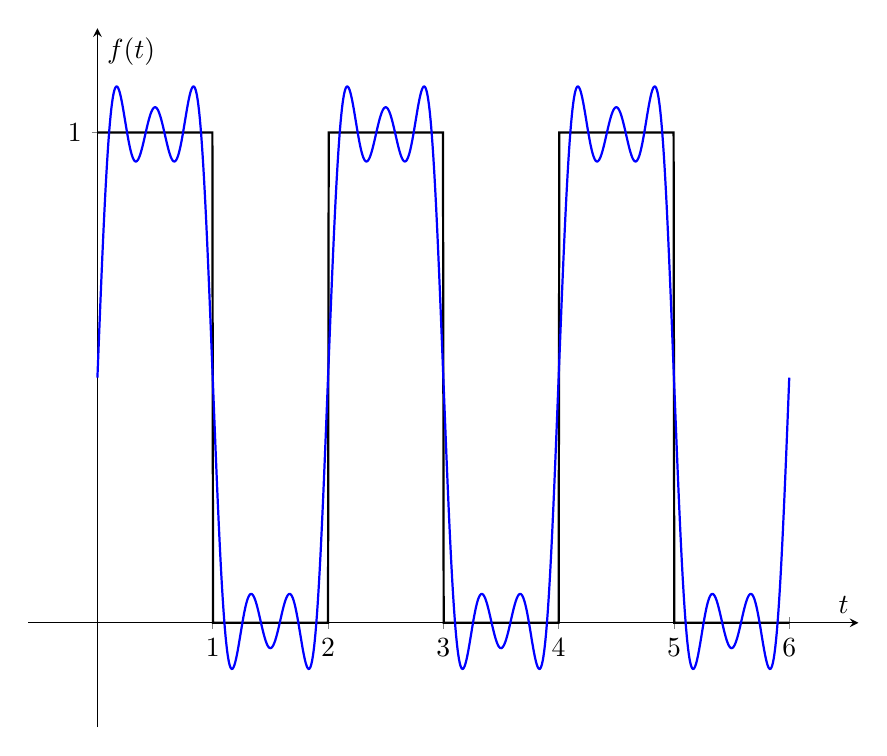
\begin{tikzpicture}
	\begin{axis}[
		axis lines = middle,
		xlabel = {$t$},
		ylabel = {$f(t)$},		
		domain=0:6,
		samples=1000,
		xtick={0,1,2,3,4,5,6},
		ytick={0,1},
		enlargelimits,
		width=\textwidth
		]
		\addplot[thick] {mod(floor(x),2) == 0 ? 1 : 0};
		\addplot[blue, thick] {(1/2) + 
			(2/pi)*sin(pi * deg(x)) + 
			(2/(3*pi))*sin(pi *3*deg(x)) +
			(2/(5*pi))*sin(pi *5*deg(x))};
	\end{axis}
\end{tikzpicture}

$a_0$ ist bei 


\subsection{Fouriertransformation\label{fourier:subsection:fouriertransformation}}


%
% teil1.tex -- Beispiel-File für das Paper
%
% (c) 2020 Prof Dr Andreas Müller, Hochschule Rapperswil
%
% !TEX root = ../../buch.tex
% !TEX encoding = UTF-8
%
\section{Metrik und Hodge-Theorie 
\label{maxwell:section:teil1}}
\kopfrechts{Metrik und Hodge-Theorie}

\subsection{Minkowski Metrik}
In der speziellen Relativitätstheorie (SRT) wird die Minkowski-Metrik verwendet.
\index{spezielle Relativitätstheorie}%
\index{Relativitätstheorie, spezielle}%
\index{Minkowski-Metrik}%
Da es in der SRT keine Krümmung und Gravitation gibt, sind alle Elemente ausserhalb der Diagonale des metrischen Tensors null und somit ist die Raum-Zeit flach.
Zwei Signaturen sind üblich.
Einerseits gibt es die $({-}{+}{+}{+})$-Signatur, bei welcher die Zeitkomponente negativ und die Raumkomponenten positiv gezählt werden.
Andererseits gibt es die $({+}{-}{-}{-})$-Signatur, bei welcher die Zeitkomponente positiv und die Raumkomponenten negativ gezählt werden.
Beide Signaturen sind gleichwertig, solange man sich auf eine Metrik festlegt und diese konsequent beibehält.
Im Folgenden werden wir uns an die $({-}{+}{+}{+})$-Signatur halten.
Daher definieren wir den metrischen Tensor als
\begin{equation}
	g^{ik} = \begin{pmatrix}
		-1 & 0 & 0 & 0 \\ 0 & 1 & 0 & 0 \\ 0 & 0 & 1 & 0 \\ 0 & 0 & 0 & 1 
	\end{pmatrix}.
	\label{maxwell:section:teil1:metrik}
\end{equation}
Der Ausdruck für ein Linienelement in dieser Metrik ist definiert als
\begin{equation*}
	dl^2 = -(dx^0)^2 +(dx^1)^2+(dx^2)^2+(dx^3)^2.
\end{equation*}
Damit wir Raum und Zeit in dieser Metrik gleichartig behandeln können, wählen wir beim Übergang in physikalische Einheiten 
\begin{equation}
	\label{maxwell:koordinaten}
	x^0 = ct,\quad x^1 = x,\quad x^2 = y, \quad x^3 = z .
\end{equation}
Dabei entspricht $c$ der Lichtgeschwindigkeit und ein Linienelement ist somit definiert als
\begin{equation*}
	dl^2 = -c^2dt^2 +dx^2+dy^2+dz^2.
\end{equation*}
Eine Konsequenz dieser Signatur ist, dass zeitartige Abstände $dl^2 < 0$ und raumartige Abstände $dl^2 > 0$ sind.

\subsection{Hodge-Duale der Basis-$k$-Formen}
Für den Teil der inhomogenen Maxwell-Gleichungen benötigen wir die Hodge-Duale von 1-Formen, 2-Formen und 3-Formen im vierdimensionalen Minkowski-Raum.
Um dabei die korrekten Vorzeichen zu erhalten, muss die Hodge-Dualität mit Hilfe des metrischen Tensors $g^{ik}$  der Minkowski-Metrik verwendet werden.

Wir verwenden die Definition des Hodge-Operators
\begin{equation*}
	\alpha \wedge \ast \beta = \langle \alpha, \beta \rangle \operatorname{vol}(M),
\end{equation*}
wobei $\langle \cdot , \cdot \rangle$ das durch die Metrik $g^{ik}$ induzierte Skalarprodukt ist.
Im Folgenden führen wir alle Berechnungen der Hodge-Duale von 1-, 2- und 3-Formen durch.
Wir verwenden $g^{ik}$ gemäss \eqref{maxwell:section:teil1:metrik} und $\operatorname{vol}(M) = dx^0 \wedge dx^1 \wedge dx^2 \wedge dx^3$.
\begin{definition}
\label{maxwell:hodge:kurzschreibweise}
Um die Notation kompakter und übersichtlicher zu gestalten, führen wir die Schreibweise
\begin{align*}
	dx^{i\!j} &:= dx^i \wedge dx^j, 
	%\label{maxwell:hodge:zwei}
	\\
	dx^{i\!jk} &:= dx^i \wedge dx^j \wedge dx^k, 
	%\label{maxwell:hodge:drei}
	\\
	dx^{i\!jkl} & := dx^i \wedge dx^j \wedge dx^k \wedge dx^l
	\notag
\end{align*}
für Wedge-Produkte von Basisformen ein.
\end{definition}
Mit dieser Vorbereitung können wir nun die konkreten Hodge-Duale der Basisformen berechnen.
\subsubsection{Hodge-Duale von 1-Formen}
\begin{align*}
	\ast dx^0 
	&= s \, dx^{123} \\
	dx^0 \wedge \ast dx^0 
	&= dx^0 \wedge s \, dx^{123} = s \, dx^{0123} \\
	&= \langle dx^0, dx^0 \rangle \operatorname{vol}(M) = g^{00} \, dx^{0123} = -dx^{0123} \\
	\Rightarrow s &= -1 \Rightarrow \boxed{\ast dx^0 = - dx^{123}}
	\\[1em]
	\ast dx^1 
	&= s \, dx^{023} \\
	dx^1 \wedge \ast dx^1 
	&= dx^1 \wedge s \, dx^{023} = -s \, dx^{0123} \\
	&= \langle dx^1, dx^1 \rangle \operatorname{vol}(M) = g^{11} \, dx^{0123} = dx^{0123} \\
	\Rightarrow s &= -1 \Rightarrow \boxed{\ast dx^1 = - dx^{023}}
	\\[1em]
	\ast dx^2 
	&= s \, dx^{013} \\
	dx^2 \wedge \ast dx^2 
	&= dx^2 \wedge s \, dx^{013} = s \, dx^{0123} \\
	&= \langle dx^2, dx^2 \rangle \operatorname{vol}(M) = g^{22} \, dx^{0123} = dx^{0123} \\
	\Rightarrow s &= +1 \Rightarrow \boxed{\ast dx^2 = dx^{013}}
	\\[1em]
	\ast dx^3 
	&= s \, dx^{012} \\
	dx^3 \wedge \ast dx^3 
	&= dx^3 \wedge s \, dx^{012} = -s \, dx^{0123} \\
	&= \langle dx^3, dx^3 \rangle \operatorname{vol}(M) = g^{33} \, dx^{0123} = dx^{0123} \\
	\Rightarrow s &= -1 \Rightarrow \boxed{\ast dx^3 = - dx^{012}}
\end{align*}

\subsubsection{Hodge-Duale von 2-Formen}
\begin{align*}
	\ast dx^{01} &= s \, dx^{23} \\
	dx^{01} \wedge \ast dx^{01} &= s \, dx^{0123} \\
	&= \langle dx^{01}, dx^{01} \rangle \, \operatorname{vol}(M) 
	= g^{00} g^{11} \operatorname{vol}(M) = -dx^{0123} \\
	\Rightarrow s &= -1 \Rightarrow \boxed{\ast dx^{01} = - dx^{23}}
	\\[1em]
	\ast dx^{12} &= s \, dx^{03} \\
	dx^{12} \wedge \ast dx^{12} &= s \, dx^{0123} \\
	&= \langle dx^{12}, dx^{12} \rangle \, \operatorname{vol}(M) 
	= g^{11} g^{22} \operatorname{vol}(M) = dx^{0123} \\
	\Rightarrow s &= +1 \Rightarrow \boxed{\ast dx^{12} = dx^{03}}
	\\[1em]
	\ast dx^{23} &= s \, dx^{01} \\
	dx^{23} \wedge \ast dx^{23} &= s \, dx^{0123} \\
	&= \langle dx^{23}, dx^{23} \rangle \, \operatorname{vol}(M) 
	= g^{22} g^{33} \operatorname{vol}(M) = dx^{0123} \\
	\Rightarrow s &= +1 \Rightarrow \boxed{\ast dx^{23} = dx^{01}}
	\\[1em]
	\ast dx^{02} &= s \, dx^{13} \\
	dx^{02} \wedge \ast dx^{02} &= -s \, dx^{0123} \\
	&= \langle dx^{02}, dx^{02} \rangle \, \operatorname{vol}(M) 
	= g^{00} g^{22} \operatorname{vol}(M) = -dx^{0123} \\
	\Rightarrow s &= +1 \Rightarrow \boxed{\ast dx^{02} = dx^{13}}
	\\[1em]
	\ast dx^{03} &= s \, dx^{12} \\
	dx^{03} \wedge \ast dx^{03} &= s \, dx^{0123} \\
	&= \langle dx^{03}, dx^{03} \rangle \, \operatorname{vol}(M) 
	= g^{00} g^{33} \operatorname{vol}(M) = -dx^{0123} \\
	\Rightarrow s &= -1 \Rightarrow \boxed{\ast dx^{03} = - dx^{12}}
	\\[1em]
	\ast dx^{13} &= s \, dx^{02} \\
	dx^{13} \wedge \ast dx^{13} &= -s \, dx^{0123} \\
	&= \langle dx^{13}, dx^{13} \rangle \, \operatorname{vol}(M) 
	= g^{11} g^{33} \operatorname{vol}(M) = dx^{0123} \\
	\Rightarrow s &= -1 \Rightarrow \boxed{\ast dx^{13} = - dx^{02}}
\end{align*}

\subsubsection{Hodge-Duale von 3-Formen}
\begin{align*}
	\ast dx^{012} &= s \, dx^3 \\
	dx^{012} \wedge \ast dx^{012} &= s \, dx^{0123} \\
	&= \langle dx^{012}, dx^{012} \rangle \, \operatorname{vol}(M) 
	= g^{00} g^{11} g^{22} \operatorname{vol}(M) = -dx^{0123} \\
	\Rightarrow s &= -1 \Rightarrow \boxed{\ast dx^{012} = - dx^3}
	\\[1em]
	\ast dx^{013} &= s \, dx^2 \\
	dx^{013} \wedge \ast dx^{013} &= -s \, dx^{0123} \\
	&= \langle dx^{013}, dx^{013} \rangle \, \operatorname{vol}(M) 
	= g^{00} g^{11} g^{33} \operatorname{vol}(M) = -dx^{0123} \\
	\Rightarrow s &= 1 \Rightarrow \boxed{\ast dx^{013} = dx^2}
	\\[1em]
	\ast dx^{023} &= s \, dx^1 \\
	dx^{023} \wedge \ast dx^{023} &= s \, dx^{0123} \\
	&= \langle dx^{023}, dx^{023} \rangle \, \operatorname{vol}(M) 
	= g^{00} g^{22} g^{33} \operatorname{vol}(M) = -dx^{0123} \\
	\Rightarrow s &= -1 \Rightarrow \boxed{\ast dx^{023} = - dx^1}
	\\[1em]
	\ast dx^{123} &= s \, dx^0 \\
	dx^{123} \wedge \ast dx^{123} &= -s \, dx^{0123} \\
	&= \langle dx^{123}, dx^{123} \rangle \, \operatorname{vol}(M)
	= g^{11} g^{22} g^{33} \operatorname{vol}(M) = dx^{0123} \\
	\Rightarrow s &= -1 \Rightarrow \boxed{\ast dx^{123} = - dx^0}
\end{align*}
In der Tabelle \ref{maxwell:section:teil1:Hodge-Tabelle} sind alle berechneten Hodge-Duale noch einmal zusammengefasst.
\begin{table}
	\centering
	%\caption{Hodge-Duale}
	%\label{maxwell:section:teil1:Hodge-Tabelle}
	\begin{tabularx}{\textwidth}{ 
			| >{\centering\arraybackslash}X 
			| >{\centering\arraybackslash}X 
			| >{\centering\arraybackslash}X | }
		\hline
		\textbf{1-Form} & \textbf{2-Form} & \textbf{3-Form} \\
		\hline
		\( \rule{0pt}{1.5em} {\ast} dx^0 = -dx^1 \wedge dx^2 \wedge dx^3 \) \newline
	\( {\ast} dx^1 = -dx^0 \wedge dx^2 \wedge dx^3 \) \newline
	\( {\ast} dx^2 = \phantom{-} dx^0 \wedge dx^1 \wedge dx^3 \) \newline
	\( {\ast} dx^3 = -dx^0 \wedge dx^1 \wedge dx^2 \, \) 
	&
	\( \rule{0pt}{1.5em} {\ast} (dx^0 \wedge dx^1) = -dx^2 \wedge dx^3 \) \newline
	\( {\ast} (dx^1 \wedge dx^2) = \phantom{-} dx^0 \wedge dx^3 \) \newline
	\( {\ast} (dx^2 \wedge dx^3) = \phantom{-} dx^0 \wedge dx^1 \) \newline
	\( {\ast} (dx^0 \wedge dx^2) = \phantom{-} dx^1 \wedge dx^3 \) \newline
	\( {\ast} (dx^0 \wedge dx^3) = -dx^1 \wedge dx^2 \) \newline
	\( {\ast} (dx^1 \wedge dx^3) = -dx^0 \wedge dx^2 \)
	&
	\( \rule{0pt}{1.5em} {\ast} (dx^0 \wedge dx^1 \wedge dx^2) = -dx^3 \) \newline
	\( {\ast} (dx^0 \wedge dx^1 \wedge dx^3) = \phantom{-} dx^2 \) \newline
	\( {\ast} (dx^0 \wedge dx^2 \wedge dx^3) = -dx^1 \) \newline
	\( {\ast} (dx^1 \wedge dx^2 \wedge dx^3) = -dx^0 \)
		\\
		\hline
	\end{tabularx}
	\caption{Tabelle aller Hodge-Duale von 1-, 2-, und 3-Formen mit $({-}{+}{+}{+})$-Signatur}
	\label{maxwell:section:teil1:Hodge-Tabelle}
\end{table}








%
% teil2.tex -- Beispiel-File für teil2 
%
% (c) 2020 Prof Dr Andreas Müller, Hochschule Rapperswil
%
% !TEX root = ../../buch.tex
% !TEX encoding = UTF-8
%
\section{Vorgeschriebene gausssche Krümmung
\label{mongeampere:section:teil2}}
\kopfrechts{Teil 2}
Mit der Definition der gausschen Krümmung können wir nun eine Differentialgleichung aufstellen,
welche als Lösung eine Fläche mit einer gewünschten gausschen Krümmung hat.
Dafür nehmen wir die explizite Form einer Fläche $z = f(x,y)$.
Die Variablen sind nun nicht mehr $u, v$ sondern $x, y$.
Nun brauchen wir die Koeffizienten der Fundamentalformen, welche mit dem Radiusvektor $\vec r$ und seinen Ableitungen 
beschrieben werden können
\begin{align}
  \vec r &= \begin{pmatrix}
   x \\
   y \\
   f(x, y)
 \end{pmatrix} \\
    \vec r_x &= \begin{pmatrix}
      1 \\
      0 \\
      \frac{\partial f}{\partial x}
    \end{pmatrix},
      \quad &
    \vec r_y &= \begin{pmatrix}
      0 \\
      1 \\
      \frac{\partial f}{\partial y}
    \end{pmatrix}\\
      \vec r_{xx} &= \begin{pmatrix}
      0 \\
      0 \\
      \frac{\partial^2 f}{\partial x^2}
    \end{pmatrix},
    \quad &
    \vec r_{xy} &= \begin{pmatrix}
      0 \\
      0 \\
      \frac{\partial^2 f}{\partial x \, \partial y}
    \end{pmatrix},
      \quad &
    \vec r_{yy} &= \begin{pmatrix}
      0 \\
      0 \\
      \frac{\partial^2 f}{\partial y^2}
    \end{pmatrix}\\
\end{align}
Damit sind die Koeffizienten der ersten Fundamentalform 
\begin{equation}
  E = 1 + \left(\frac{\partial f}{\partial x}\right)^2, \quad
  F = \frac{\partial f}{\partial x} \cdot \frac{\partial f}{\partial y}, \quad
  G = 1 + \left(\frac{\partial f}{\partial y}\right)^2
  \label{mongeampere:fund1exp}
\end{equation}
Für die zweite Fundamentalform wird die Flächennormale benötigt, welche aus \eqref{mongeampere:norm} und \eqref{mongeampere:ds} 
\begin{equation}
  \vec m = \frac{\vec r_x \times \vec r_y}{\sqrt{EG-F^2}} = \begin{pmatrix}
    \frac{\partial f}{\partial x} \\
    \frac{\partial f}{\partial y} \\
    1
  \end{pmatrix}
  \frac{1}{\sqrt{EG-F^2}}
  \label{mongeampere:norm2}
\end{equation}
ist.
Somit sind die Koeffizienten der zweiten Fundamentalform
\begin{equation}
  L = \frac{\frac{\partial^2 f}{\partial x^2}}{\sqrt{EG-F}}, \quad
  M = \frac{\frac{\partial^2 f}{\partial x \, \partial y}}{\sqrt{EG-F}}, \quad
  N = \frac{\frac{\partial^2 f}{\partial y^2}}{\sqrt{EG-F}}
  \label{mongeampere:2fund22}
\end{equation}
Setzen wir die Koeffizienten aus \eqref{mongeampere:fund1exp} und \eqref{mongeampere:2fund22} in die Formel der gausschen Krümmung \eqref{mongeampere:gausskrumm}
ein, erhalten wir
\begin{equation}
  K = \frac{
    \frac{\partial^2 f}{\partial x^2} \cdot \frac{\partial^2 f}{\partial y^2} - \left(\frac{\partial^2 f}{\partial x \, \partial y} \right)^2}
    {\left[1 + 
    \left(\frac{\partial f}{\partial x}\right)^2 +
    \left(\frac{\partial f}{\partial y}\right)^2\right]^2}.
  \label{mongeampere:pd}
\end{equation}
Wie wir sehen können, ist der Zähler gleich der Determinante der hesseschen Matrix von $f(x,y)$.
Der Nenner ist eine nichtlineare Funktion der ersten Ableitungen.
Somit konnten wir zeigen, dass das Prescribed Gaussian Curvature Problem einer explizit definierten Fläche in einer 
monge-ampèreschen Gleichung resultiert.


%
% teil3.tex -- Beispiel-File für Teil 3
%
% (c) 2020 Prof Dr Andreas Müller, Hochschule Rapperswil
%
% !TEX root = ../../buch.tex
% !TEX encoding = UTF-8
%
\section{Teil 3
\label{ueberschall:section:teil3}}
\kopfrechts{Teil 3}
Sed ut perspiciatis unde omnis iste natus error sit voluptatem
accusantium doloremque laudantium, totam rem aperiam, eaque ipsa
quae ab illo inventore veritatis et quasi architecto beatae vitae
dicta sunt explicabo. Nemo enim ipsam voluptatem quia voluptas sit
aspernatur aut odit aut fugit, sed quia consequuntur magni dolores
eos qui ratione voluptatem sequi nesciunt. Neque porro quisquam
est, qui dolorem ipsum quia dolor sit amet, consectetur, adipisci
velit, sed quia non numquam eius modi tempora incidunt ut labore
et dolore magnam aliquam quaerat voluptatem. Ut enim ad minima
veniam, quis nostrum exercitationem ullam corporis suscipit laboriosam,
nisi ut aliquid ex ea commodi consequatur? Quis autem vel eum iure
reprehenderit qui in ea voluptate velit esse quam nihil molestiae
consequatur, vel illum qui dolorem eum fugiat quo voluptas nulla
pariatur?

\subsection{De finibus bonorum et malorum
\label{ueberschall:subsection:malorum}}
At vero eos et accusamus et iusto odio dignissimos ducimus qui
blanditiis praesentium voluptatum deleniti atque corrupti quos
dolores et quas molestias excepturi sint occaecati cupiditate non
provident, similique sunt in culpa qui officia deserunt mollitia
animi, id est laborum et dolorum fuga. Et harum quidem rerum facilis
est et expedita distinctio. Nam libero tempore, cum soluta nobis
est eligendi optio cumque nihil impedit quo minus id quod maxime
placeat facere possimus, omnis voluptas assumenda est, omnis dolor
repellendus. Temporibus autem quibusdam et aut officiis debitis aut
rerum necessitatibus saepe eveniet ut et voluptates repudiandae
sint et molestiae non recusandae. Itaque earum rerum hic tenetur a
sapiente delectus, ut aut reiciendis voluptatibus maiores alias
consequatur aut perferendis doloribus asperiores repellat.




\printbibliography[heading=subbibliography]
\end{refsection}
